\documentclass[conference]{IEEEtran}

\usepackage{graphicx}
\usepackage{amsmath}
\usepackage{cite}
\usepackage{booktabs}

\title{Resource-Efficient Software Vulnerability Detection
Using Fine-Tuned Code Large Language Models }

\author{
\IEEEauthorblockN{Rohan, Sariga Saji, Vaasanth, Gopakumar.G, M.S Basanth}
\IEEEauthorblockA{
Department of Computer Science and Engineering (AI)\\
Amrita Vishwa Vidyapeetham,Amritapuri,India\\
}
}

\begin{document}
\maketitle

% =====================================================
\begin{abstract}
Software vulnerability detection is critical for secure software development, yet traditional static analysis tools often struggle with false positives and limited generalization. This paper presents a transformer-based framework for multi-class Common Weakness Enumeration (CWE) classification using lightweight encoder models on the Juliet C/C++ Test Suite. A key contribution is a template-aware dataset splitting strategy that prevents structural data leakage between training and testing samples, enabling more reliable evaluation than conventional random splitting. To address severe class imbalance, weighted cross-entropy loss is incorporated during training. Multiple transformer architectures including RoBERTa, CodeBERT, and CodeT5 are comparatively evaluated for CWE classification. Experimental results show that fine-tuned transformer models achieve strong vulnerability classification performance, with the proposed CodeT5-small model achieving a macro-F1 score of 0.9605 under template-aware evaluation. Ablation analysis confirms that random dataset splitting artificially inflates performance compared to template-aware evaluation. The findings demonstrate that compact transformer models provide an efficient and practical solution for automated vulnerability detection in secure software development workflows.
\end{abstract}

\begin{IEEEkeywords}
CodeT5, CWE Classification, Vulnerability Detection, Transformers, Software Security
\end{IEEEkeywords}

% =====================================================
\section{Introduction}

Software vulnerabilities are increasing with system complexity. As software applications grow more interconnected and development cycles shorten, vulnerabilities introduced early in the development process can reach production systems with little to no manual inspection. This makes automated identification of software weaknesses a critical element of secure software development practices.

Static Application Security Testing (SAST) tools that analyze source code without execution are widely used in the industry. However, traditional rule-based and signature-driven approaches depend heavily on pre-defined patterns, severely restricting their capability to generalize to newly discovered or modified coding weaknesses. Furthermore, such tools often produce high false-positive rates, which erode developer trust and impede integration into agile development workflows.

Recent cybersecurity research from Amrita Vishwa Vidyapeetham has explored machine learning and deep learning approaches for intrusion detection, malware analysis, and intelligent cyber defense systems, highlighting the growing role of AI-driven security analytics in software protection~\cite{amrita1,amrita2,amrita3,amrita4,amrita5,amrita6}.

Transformer-based models have recently demonstrated strong performance in source code understanding and vulnerability detection tasks due to their ability to capture contextual relationships within code sequences. However, ensuring reliable evaluation remains a significant challenge, particularly when benchmark datasets contain structurally similar template-generated samples that may introduce structural data leakage between training and testing sets.

This work investigates whether compact transformer architectures can provide an effective balance between vulnerability classification performance and computational efficiency for CWE detection. To improve evaluation reliability, we introduce a template-aware dataset splitting strategy that prevents structural leakage between training and testing samples. Multiple transformer-based encoder models are evaluated for CWE classification across 118 vulnerability categories using the Juliet benchmark dataset.

This paper makes the following contributions:
\begin{itemize}
    \item We propose a template-aware dataset splitting strategy that prevents structural data leakage and enables more reliable evaluation for CWE vulnerability classification.
    
    \item We perform a comparative evaluation of transformer-based encoder models including RoBERTa, CodeBERT, CodeT5-base, and CodeT5-small for multi-class CWE classification across 118 vulnerability categories.

    \item We address severe dataset imbalance through weighted loss optimization and analyze model behavior using macro-level evaluation metrics, confusion analysis, and class-wise performance trends.

    \item We demonstrate the practical viability of compact transformer-based vulnerability detection through performance, efficiency, and generalization analysis.
\end{itemize}
% =====================================================
\section{Related Work}

Early software vulnerability detection approaches primarily relied on static analysis techniques such as rule-based pattern matching and symbolic execution. While effective at identifying known vulnerability patterns, these approaches often struggled to generalize to unseen weaknesses and were prone to high false-positive rates.

With the growth of machine learning, vulnerability detection began to be modeled as a supervised learning problem. VulDeePecker~\cite{vuldee} demonstrated that neural networks could effectively detect vulnerabilities by learning from extracted code gadgets. Subsequent representation learning approaches such as Code2Vec~\cite{code2vec} and CC2Vec~\cite{cc2vec} focused on learning semantic embeddings from token sequences and syntactic structures. Although these methods improved automated vulnerability analysis, they remained limited in capturing long-range dependencies and deeper contextual relationships in source code.

Transformer-based architectures significantly advanced source code understanding by leveraging self-attention mechanisms to model global program context. Models such as CodeBERT~\cite{codebert}, GraphCodeBERT~\cite{graphcodebert}, and CodeT5~\cite{codet5} have demonstrated strong performance across vulnerability detection, defect prediction, and code intelligence tasks. Empirical analyses~\cite{chen2022,msr2020} further suggest that transformer architectures provide substantial gains in code modeling compared to earlier neural approaches.

Parallel cybersecurity research, including contributions from Amrita Vishwa Vidyapeetham, has highlighted the effectiveness of deep learning techniques for cyber threat analysis, intrusion detection, and intelligent security monitoring~\cite{amrita1,amrita2}. These studies reinforce the broader applicability of machine learning-driven security analytics.

This work addresses these limitations through comparative evaluation of transformer-based architectures combined with a template-aware dataset splitting strategy for more reliable multi-class CWE classification evaluation.

% =====================================================
\section{Dataset and Proposed Method}
\subsection{Overview of Juliet Test Suite}

The Juliet Test Suite is a benchmark dataset developed for evaluating software vulnerability detection systems. It contains structured examples of vulnerable and non-vulnerable code written in C and C++. Each test case consists of:
\begin{itemize}
    \item A \textit{bad} function that contains a vulnerability
    \item A \textit{good} function that provides a corrected version
    \item A CWE label indicating the vulnerability category
\end{itemize}
The dataset includes multiple template-based variations of each vulnerability type, ensuring diversity in code structure while maintaining consistent vulnerability patterns.

\subsection{Dataset Statistics}

\begin{table}[t]
\centering
\caption{Dataset statistics for the Juliet Test Suite}
\begin{tabular}{lc}
\toprule
Metric & Value \\
\midrule
Total Samples & 179,839 \\
Number of CWE Classes & 118 \\
Largest Class Size & $\sim$16,000 \\
Smallest Class Size & $<$10 \\
Language & C/C++ \\
\bottomrule
\end{tabular}
\end{table}

The dataset exhibits a highly imbalanced long-tailed distribution, where a small number of CWE categories dominate the majority of samples. This imbalance reflects the actual distribution of vulnerability types in software systems and presents a significant challenge for supervised learning models.

\subsection{Data Preprocessing}

The preprocessing stage plays a crucial role in preparing the dataset for training. The following steps are applied:
\begin{enumerate}
    \item Removal of redundant whitespace
    \item Preservation of comments to retain semantic context
    \item Conversion of code into a normalized format
    \item Tokenization using the CodeT5 tokenizer with a maximum sequence length of 256 tokens
    In addition, code tokens are processed using a subword tokenization scheme, allowing the model to handle rare identifiers and unseen tokens effectively. Comments are retained as they often contain semantic hints about program intent, which can assist in vulnerability detection. For code samples exceeding the maximum sequence length, truncation is applied, which may lead to partial context loss but ensures computational efficiency and uniform input size.
\end{enumerate}
These steps ensure that the model receives consistent and meaningful input representations.

\subsection{Template-Aware Dataset Splitting Strategy}

The Juliet Test Suite presents a significant challenge through its template-based code generation. Samples share a common vulnerability template but differ through minor code changes. A naive random split can place structurally similar samples in both training and testing sets, leading to inflated performance metrics due to memorized patterns rather than genuine generalization capability.

To address this, a template-aware splitting strategy is introduced. All samples generated from a single vulnerability template are assigned to either the training set or the testing set exclusively, creating complete structural separation. This approach reduces structural overlap between training and testing samples, providing a more reliable evaluation than conventional random splitting.


\subsection{Model Architecture}

CodeT5-small is used as the backbone model due to its efficiency and strong performance on code understanding tasks. The model processes tokenized source code as input and creates contextual representations that capture both syntactic and semantic relationships between program elements.
The model takes tokenized source code as input and passes it through the encoder to generate contextual embeddings. These embeddings are aggregated and fed into a fully connected classification layer, followed by a softmax function to produce class probabilities. The choice of CodeT5-small provides a balance between computational efficiency and representational power, making it suitable for large-scale classification tasks.
The encoded representations are forwarded to a linear classification head with a softmax activation layer to produce probability scores across all 118 CWE categories. The training objective is the multi-class cross-entropy loss function:

\[
\mathcal{L} = - \sum_{i=1}^{N} y_i \log(\hat{y}_i)
\]

where $y_i$ is the ground truth label distribution and $\hat{y}_i$ is the predicted probability for class $i$.

Key characteristics of CodeT5-small:
\begin{itemize}
    \item Encoder layers: 6
    \item Attention heads: 8
    \item Hidden size: 512
    \item Parameters: $\sim$60M
\end{itemize}

\subsection{Loss Function Explanation}
The model is trained using the multi-class cross-entropy loss function, which measures the difference between predicted probabilities and actual labels.

The objective of this loss function is to minimize the error between the predicted class distribution and the true distribution. By penalizing incorrect predictions, the model learns to assign higher probabilities to the correct classes.

To mitigate severe class imbalance, class-weighted cross-entropy loss is incorporated during training. Higher weights are assigned to underrepresented CWE categories, enabling the model to penalize minority-class misclassifications more strongly and improve balanced learning across all classes, where higher importance is given to underrepresented classes. This helps improve performance across all categories, especially for rare vulnerabilities.
\begin{figure}[t]
\centering
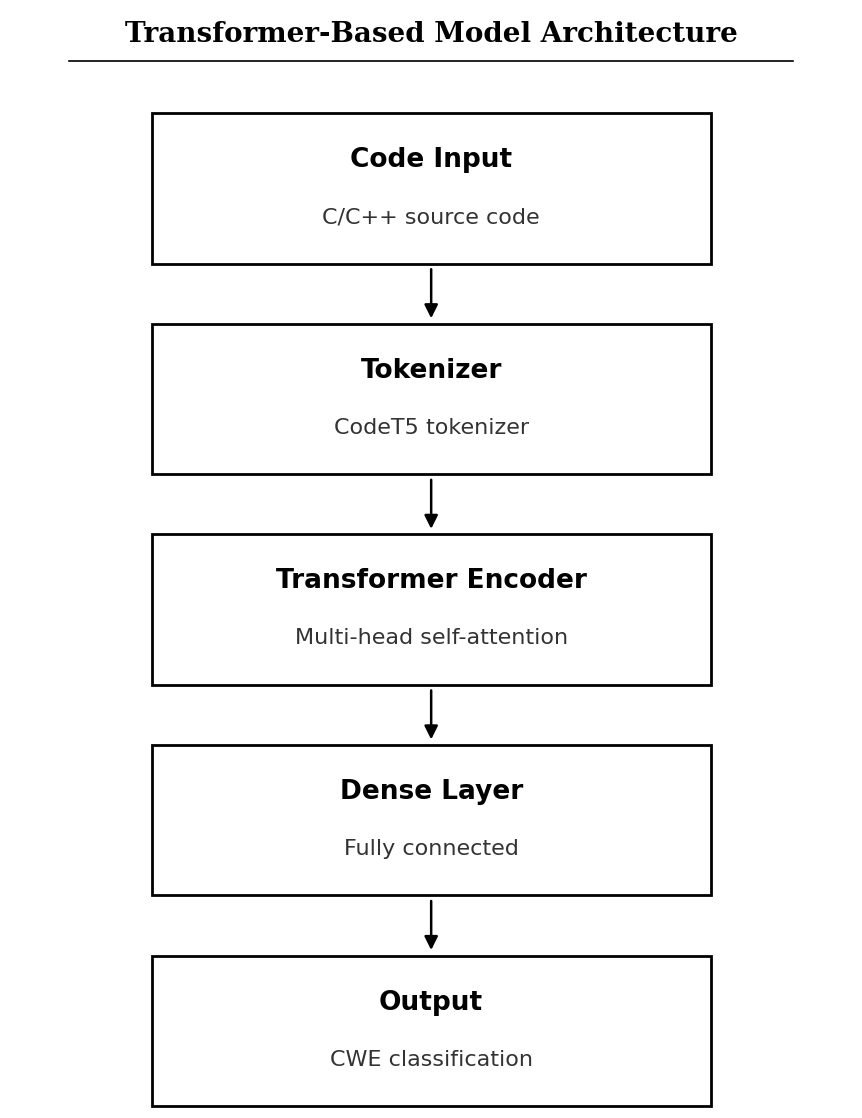
\includegraphics[width=0.48\textwidth]{architecture.png}
\caption{Overall architecture of the proposed CWE detection framework showing dataset construction, template-aware splitting, preprocessing, CodeT5 encoding, classification, and evaluation pipeline.}
\label{fig:architecture}
\end{figure}

\subsection{Training Configuration}

The model was fine-tuned using the AdamW optimizer to achieve stable parameter updates and improved generalization. The training configuration is summarized as follows:

\begin{itemize}
    \item Batch size: 4
    \item Learning rate: $5\times10^{-5}$
    \item Epochs: 2
    \item Optimizer: AdamW
\end{itemize}

Dropout regularization and early stopping were incorporated to reduce the risk of overfitting. Model performance was evaluated using accuracy, precision, recall, and macro-averaged F1-score, with macro-F1 used as the primary metric to ensure balanced evaluation across all 118 vulnerability categories despite severe class imbalance.

Training was performed on an NVIDIA GPU-equipped environment with 16 GB VRAM, with each epoch requiring approximately 2--3 hours. Training dynamics and convergence behavior are analyzed separately in Section IV-A.
% =====================================================
\section{Experimental Setup}

The Juliet Test Suite is used as the evaluation platform, which contains both vulnerable and non-vulnerable programs spanning various CWE categories.The original class distribution is maintained to preserve the inherent long-tailed vulnerability distribution present in the benchmark dataset.

The dataset used in this study contains approximately 179,839 code samples distributed across 118 CWE categories. The dataset exhibits a strong long-tailed distribution where certain vulnerability types occur frequently while most others exist in very limited quantities. The largest class contains approximately 16,000 samples while the smallest classes contain fewer than 10 samples, resulting in extreme class imbalance.

All 179,839 code samples from the Juliet Test Suite were used in this study. An 80:20 template-aware split was applied, resulting in approximately 144,000 training samples and 36,000 testing samples, with complete structural separation between the two partitions. The template-aware splitting strategy ensures that structurally similar code patterns derived from the same vulnerability template do not appear in both training and testing sets.


\subsection{Training Performance}

\begin{table}[t]
\centering
\caption{Training convergence across epochs}
\label{tab:convergence}
\begin{tabular}{lcc}
\toprule
Metric & Epoch 1 & Epoch 2 \\
\midrule
Training Loss & Decreasing & Stabilized \\
Validation Loss & Decreasing & Stabilized \\
Model Convergence & Rapid & Converged \\
\bottomrule
\end{tabular}
\end{table}
\begin{figure}[t]
\centering
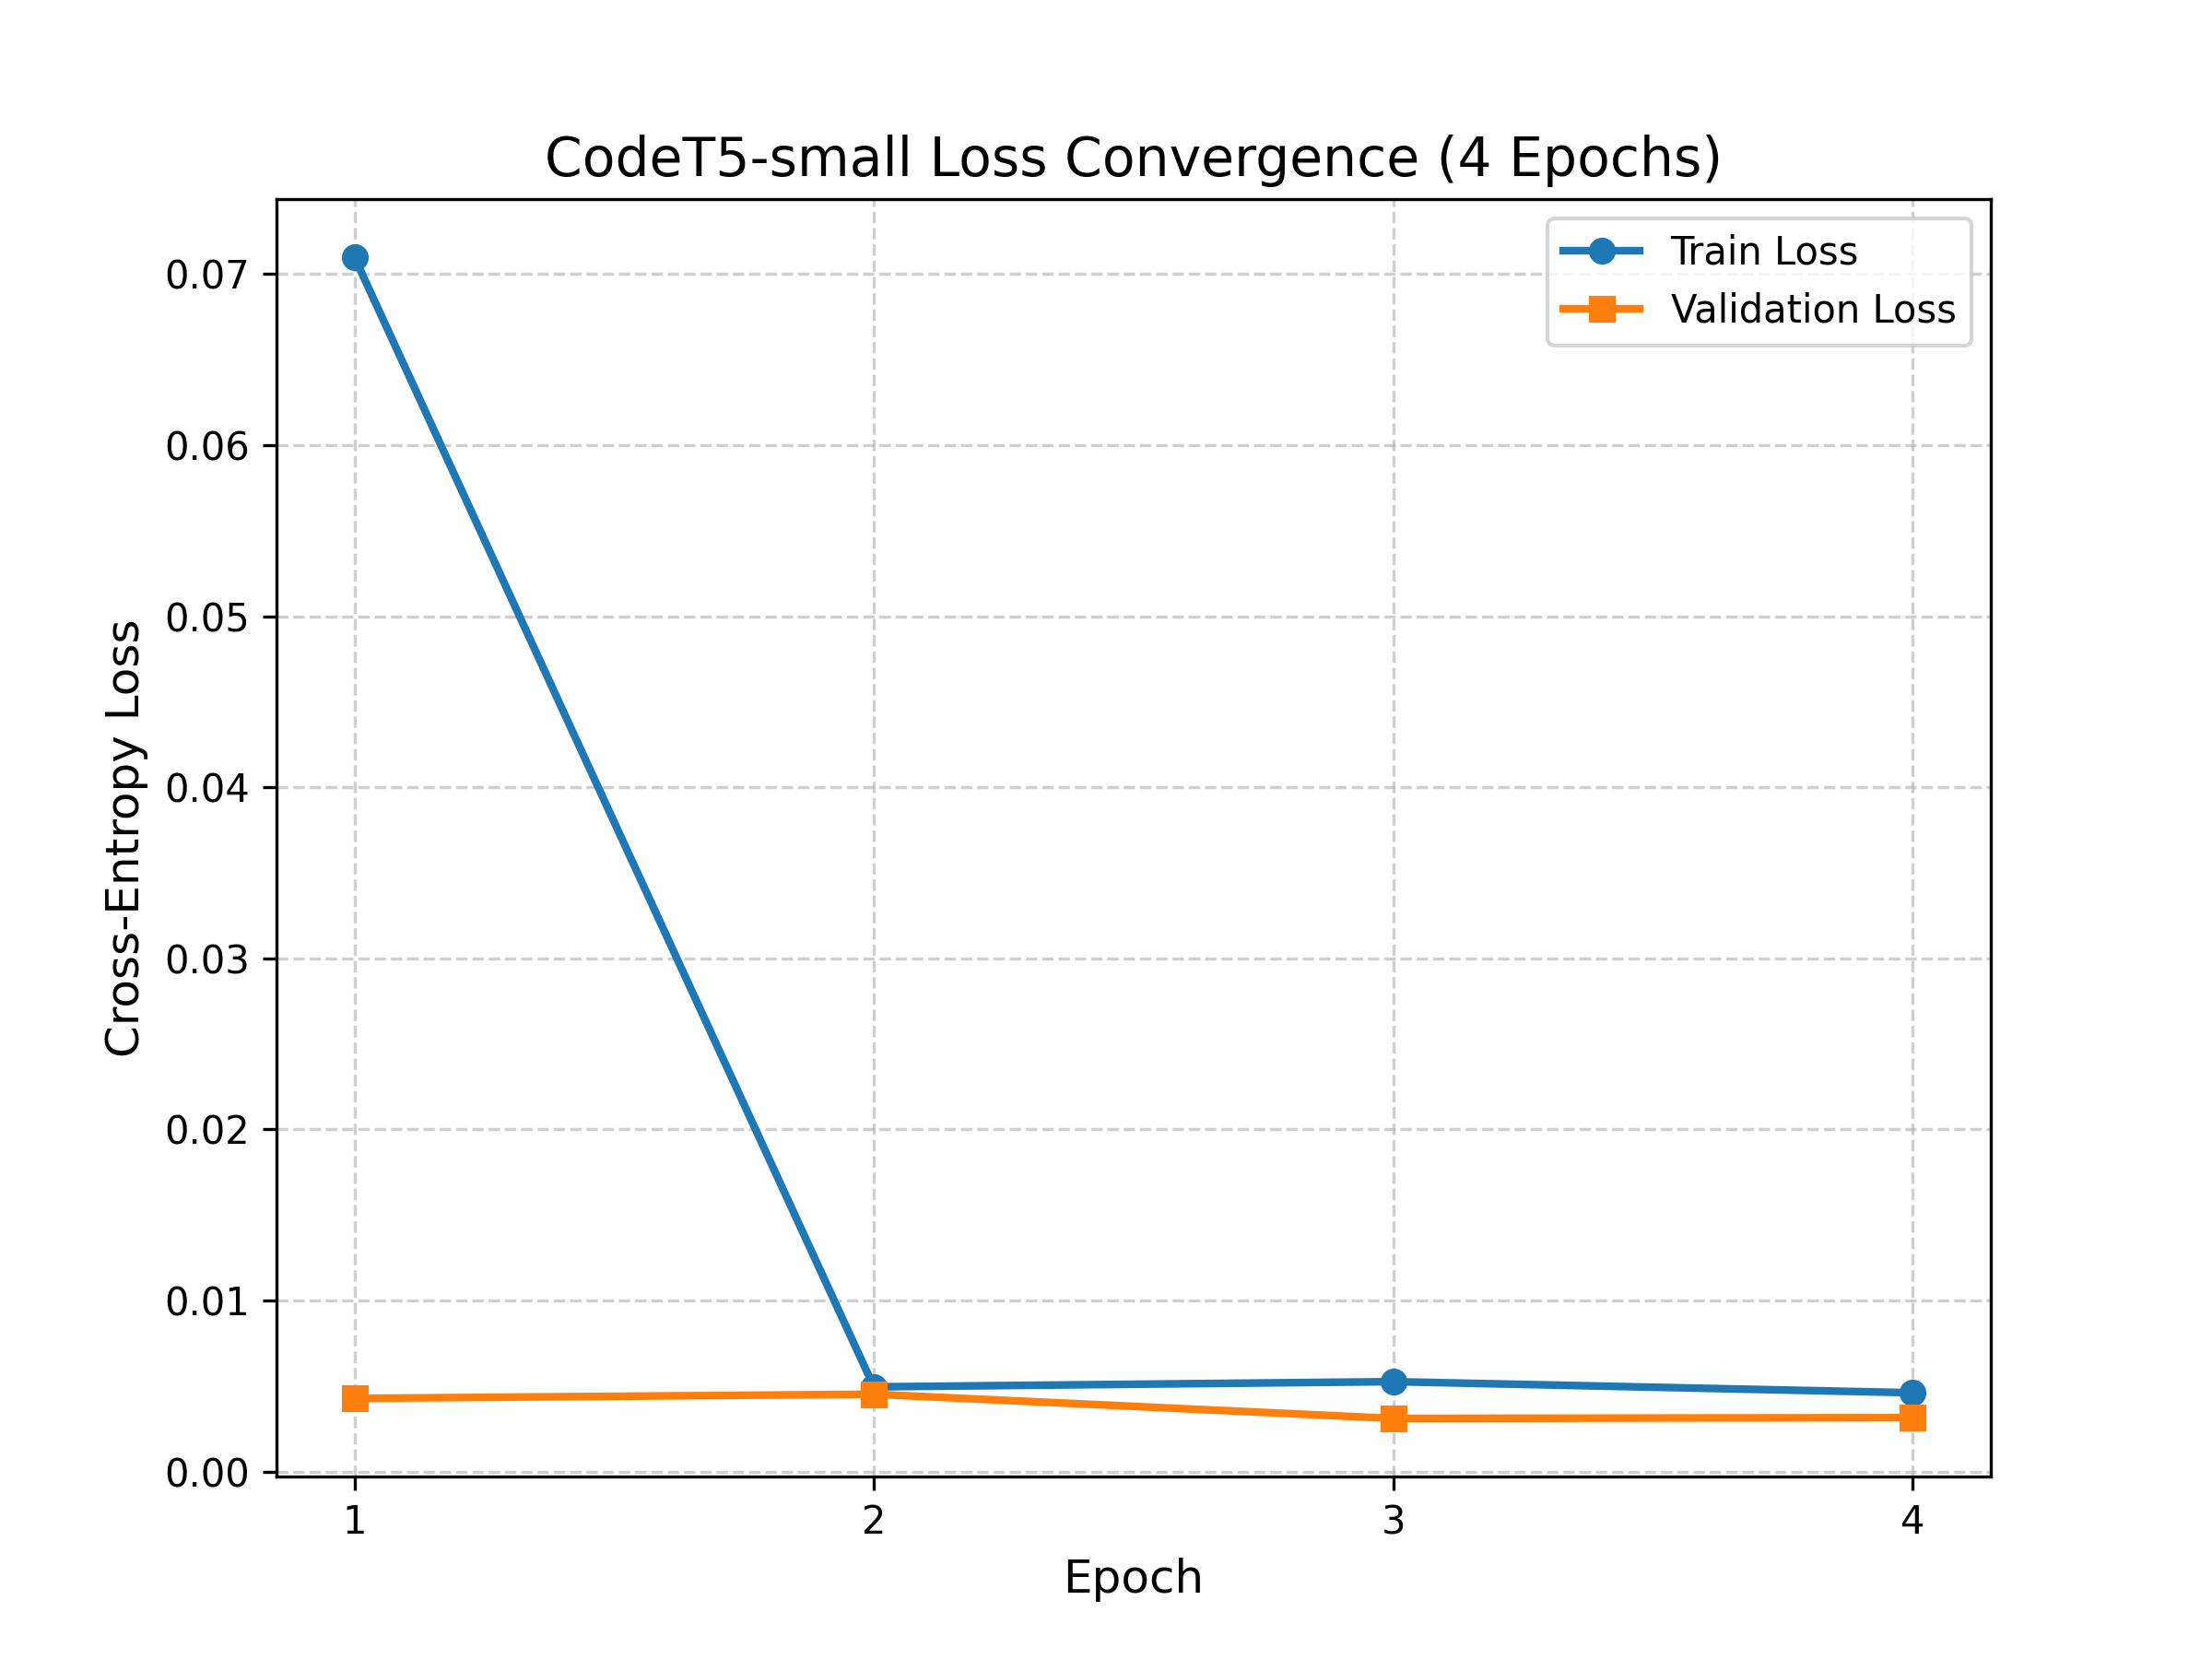
\includegraphics[width=0.48\textwidth]{codet5_4_epochs_convergence.png}
\caption{Cross-entropy loss convergence of the CodeT5-small model over four epochs. Both training and validation losses stabilize after the third epoch, indicating stable optimization behavior.}
\label{fig:loss}
\end{figure}
\subsection{Training Dynamics and Convergence Stability}

To further verify training stability, the CodeT5-small model was trained for four epochs under the same hyperparameter configuration. Figure~\ref{fig:loss} shows the training and validation loss progression.

The training loss decreases rapidly from 0.0710 to approximately 0.0045, while the validation loss stabilizes at 0.0031 by the third epoch. The absence of divergence between training and validation losses indicates stable optimization and suggests that the model does not exhibit noticeable overfitting under the current training configuration.

The loss curves plateau after the third epoch, indicating that additional training provides minimal performance gains. These observations support the selection of a small number of training epochs for efficient model convergence.

% =====================================================
As shown in Table~\ref{tab:injection}, injection-related vulnerability categories achieve particularly high precision due to their highly structured semantic patterns. OS Command Injection (CWE-78) achieved a precision of 0.9936 and an F1-score of 0.9968 across 11,884 samples, while LDAP Injection (CWE-90) achieved a precision, recall, and F1-score of 0.9981. These results indicate that the model effectively captures the characteristic execution-based patterns associated with injection vulnerabilities.

\begin{table}[t]
\centering
\caption{Performance of representative injection vulnerability categories}
\label{tab:injection}
\begin{tabular}{lccc}
\toprule
CWE & Precision & Recall & F1-score \\
\midrule
CWE-78 (OS Command Injection) & 0.9936 & 1.0000 & 0.9968 \\
CWE-90 (LDAP Injection) & 0.9981 & 0.9981 & 0.9981 \\
\bottomrule
\end{tabular}
\end{table}

The proposed CodeT5-small model achieved a macro-averaged F1-score of 96.05\% under the template-aware evaluation setting, demonstrating strong balanced classification performance across multiple CWE vulnerability categories.
\begin{table}[t]
\centering
\caption{Comparison of transformer-based models for CWE classification}
\begin{tabular}{lcc}
\toprule
Model & Parameters & Macro F1 \\
\midrule
CodeBERT & $\sim$125M & 0.9983 \\
RoBERTa & $\sim$125M & 0.9951 \\
CodeT5-base & $\sim$220M & 0.9978 \\
Proposed (CodeT5-small) & $\sim$60M & 0.9605 \\
\bottomrule
\end{tabular}
\label{tab:modelcomparison}
\end{table}

The results indicate that larger transformer architectures achieve higher classification performance, while the proposed CodeT5-small model significantly reduces parameter count and computational requirements. With approximately 60 million parameters, the proposed model requires substantially less memory than CodeBERT and CodeT5-base while still maintaining strong vulnerability classification performance under template-aware evaluation. This demonstrates the practical feasibility of lightweight transformer architectures for deployment-oriented secure software analysis workflows.

\subsection{Impact of Training Sample Size}

The number of training samples per CWE category significantly affects classification performance. Classes with larger sample sizes enable the model to learn stable and generalized representations, resulting in higher precision and lower prediction variance.

Conversely, minority classes with limited training data present a major challenge. The model struggles to learn discriminative features for these categories, leading to higher misclassification rates. This highlights the impact of long-tailed data distributions on supervised learning models.
\subsection{Precision--Recall Analysis}

Figure~\ref{fig:pr} presents the class-wise precision and recall distribution across the evaluated CWE categories. The majority of classes achieve high precision and recall, indicating that the model effectively captures common vulnerability patterns and maintains consistent classification performance across well-represented categories.

Table~\ref{tab:lowcwe} presents representative examples of vulnerability categories that achieved comparatively low F1-scores under the template-aware evaluation setting.However, a number of outlier classes exhibit substantially lower performance. As shown in Table~\ref{tab:lowcwe}, several cryptography-related vulnerability categories such as CWE-325 (Missing Required Cryptographic Step), CWE-338 (Weak Pseudo-Random Number Generator), CWE-321 (Use of Hard-coded Cryptographic Key), CWE-327 (Use of Broken/Risky Cryptographic Algorithm), and CWE-328 (Reversible One-Way Hash) achieve significantly lower F1-scores. These categories typically require deeper semantic understanding and are represented by comparatively fewer training examples.

Overall, the analysis suggests that most classification errors arise from class imbalance and limited representation of minority classes rather than instability of the underlying model architecture.
\begin{figure}[t]
\centering
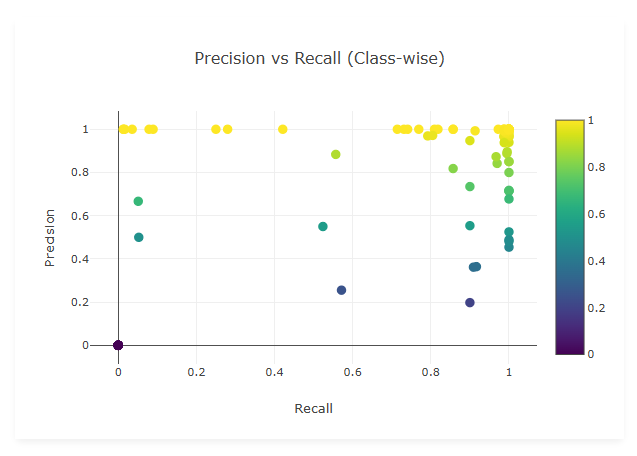
\includegraphics[width=0.48\textwidth]{precision.png}
\caption{Class-wise precision versus recall across CWE categories. Performance varies across classes, with underrepresented categories generally exhibiting larger variability.}
\label{fig:pr}
\end{figure}
\begin{table}[t]
\centering
\caption{Examples of low-performing CWE categories under template-aware evaluation}
\label{tab:lowcwe}
\begin{tabular}{lccc}
\toprule
CWE & Precision & Recall & F1-score \\
\midrule
CWE-325 & 0.0000 & 0.0000 & 0.0000 \\
CWE-338 & 0.0000 & 0.0000 & 0.0000 \\
CWE-321 & 1.0000 & 0.0167 & 0.0328 \\
CWE-327 & 1.0000 & 0.0789 & 0.1463 \\
CWE-328 & 1.0000 & 0.0357 & 0.0690 \\
\bottomrule
\end{tabular}
\end{table}
\subsection{Cross-Categorical Performance Variance}

To evaluate performance consistency across all 118 CWE categories, we computed the mean and standard deviation of the individual class-wise F1-scores.

The proposed CodeT5-small model achieved a mean class-wise F1-score of $0.9990 \pm 0.0057$.

The low standard deviation indicates that performance remains relatively consistent across most vulnerability categories and is not dominated exclusively by a small number of highly populated classes. This suggests that the model maintains stable predictive behavior across a diverse range of CWE categories despite the severe class imbalance present in the dataset.

% =====================================================
\subsection{Ablation Study: Effect of Template-Aware Splitting}

To evaluate the impact of structural data leakage, an ablation study was conducted comparing conventional random splitting with the proposed template-aware dataset partitioning strategy.

\begin{table}[t]
\centering
\caption{Ablation study on dataset splitting strategy}
\label{tab:ablation}
\begin{tabular}{lcc}
\toprule
Split Strategy & Macro F1 & Template Leakage \\
\midrule
Random Split & 0.9984 & 96.08\% \\
Template-Aware Split & 0.9605 & 0.00\% \\
\bottomrule
\end{tabular}
\end{table}

As shown in Table~\ref{tab:ablation}, conventional random splitting produces artificially inflated performance due to substantial structural overlap between training and testing samples. Approximately 96.08\% of test templates were already present in the training set under random partitioning, allowing the model to memorize template-specific code structures rather than learning generalized vulnerability semantics.

In contrast, the proposed template-aware split completely eliminates structural leakage and provides a more reliable assessment of model generalization than conventional random splitting. The observed performance gap confirms that naive random splitting can significantly overestimate vulnerability detection capability in template-generated benchmark datasets such as Juliet.
\section{Pattern and Error Analysis}

\subsection{Pattern Analysis}

Feature-based analysis reveals that different CWE classes exhibit distinct syntactic and structural patterns that the model learns to exploit:
\begin{itemize}
    \item Struct usage is strongly associated with memory-related vulnerabilities
    \item Integer constants are characteristic of overflow vulnerabilities
    \item Pointer arithmetic is indicative of memory access errors
\end{itemize}
Despite these observed patterns, the model struggles with minority classes where insufficient training examples prevent the learning of reliable decision boundaries.
For example, vulnerabilities related to buffer overflows and improper memory access are often confused due to their similar use of pointer operations and boundary conditions. Such overlaps indicate that while the model captures general patterns effectively, it struggles with fine-grained distinctions between closely related vulnerability types.
\subsection{Confusion Matrix Analysis}

The confusion matrix for the most frequently occurring CWE categories reveals that most misclassifications occur between semantically related vulnerability classes.
\begin{itemize}
    \item Majority classes dominate predictions across the dataset
    \item Minority classes are frequently misclassified due to limited training data
    \item Certain large classes consistently appear as predicted outputs for misclassified minority samples
\end{itemize}
\begin{figure}[t]
\centering
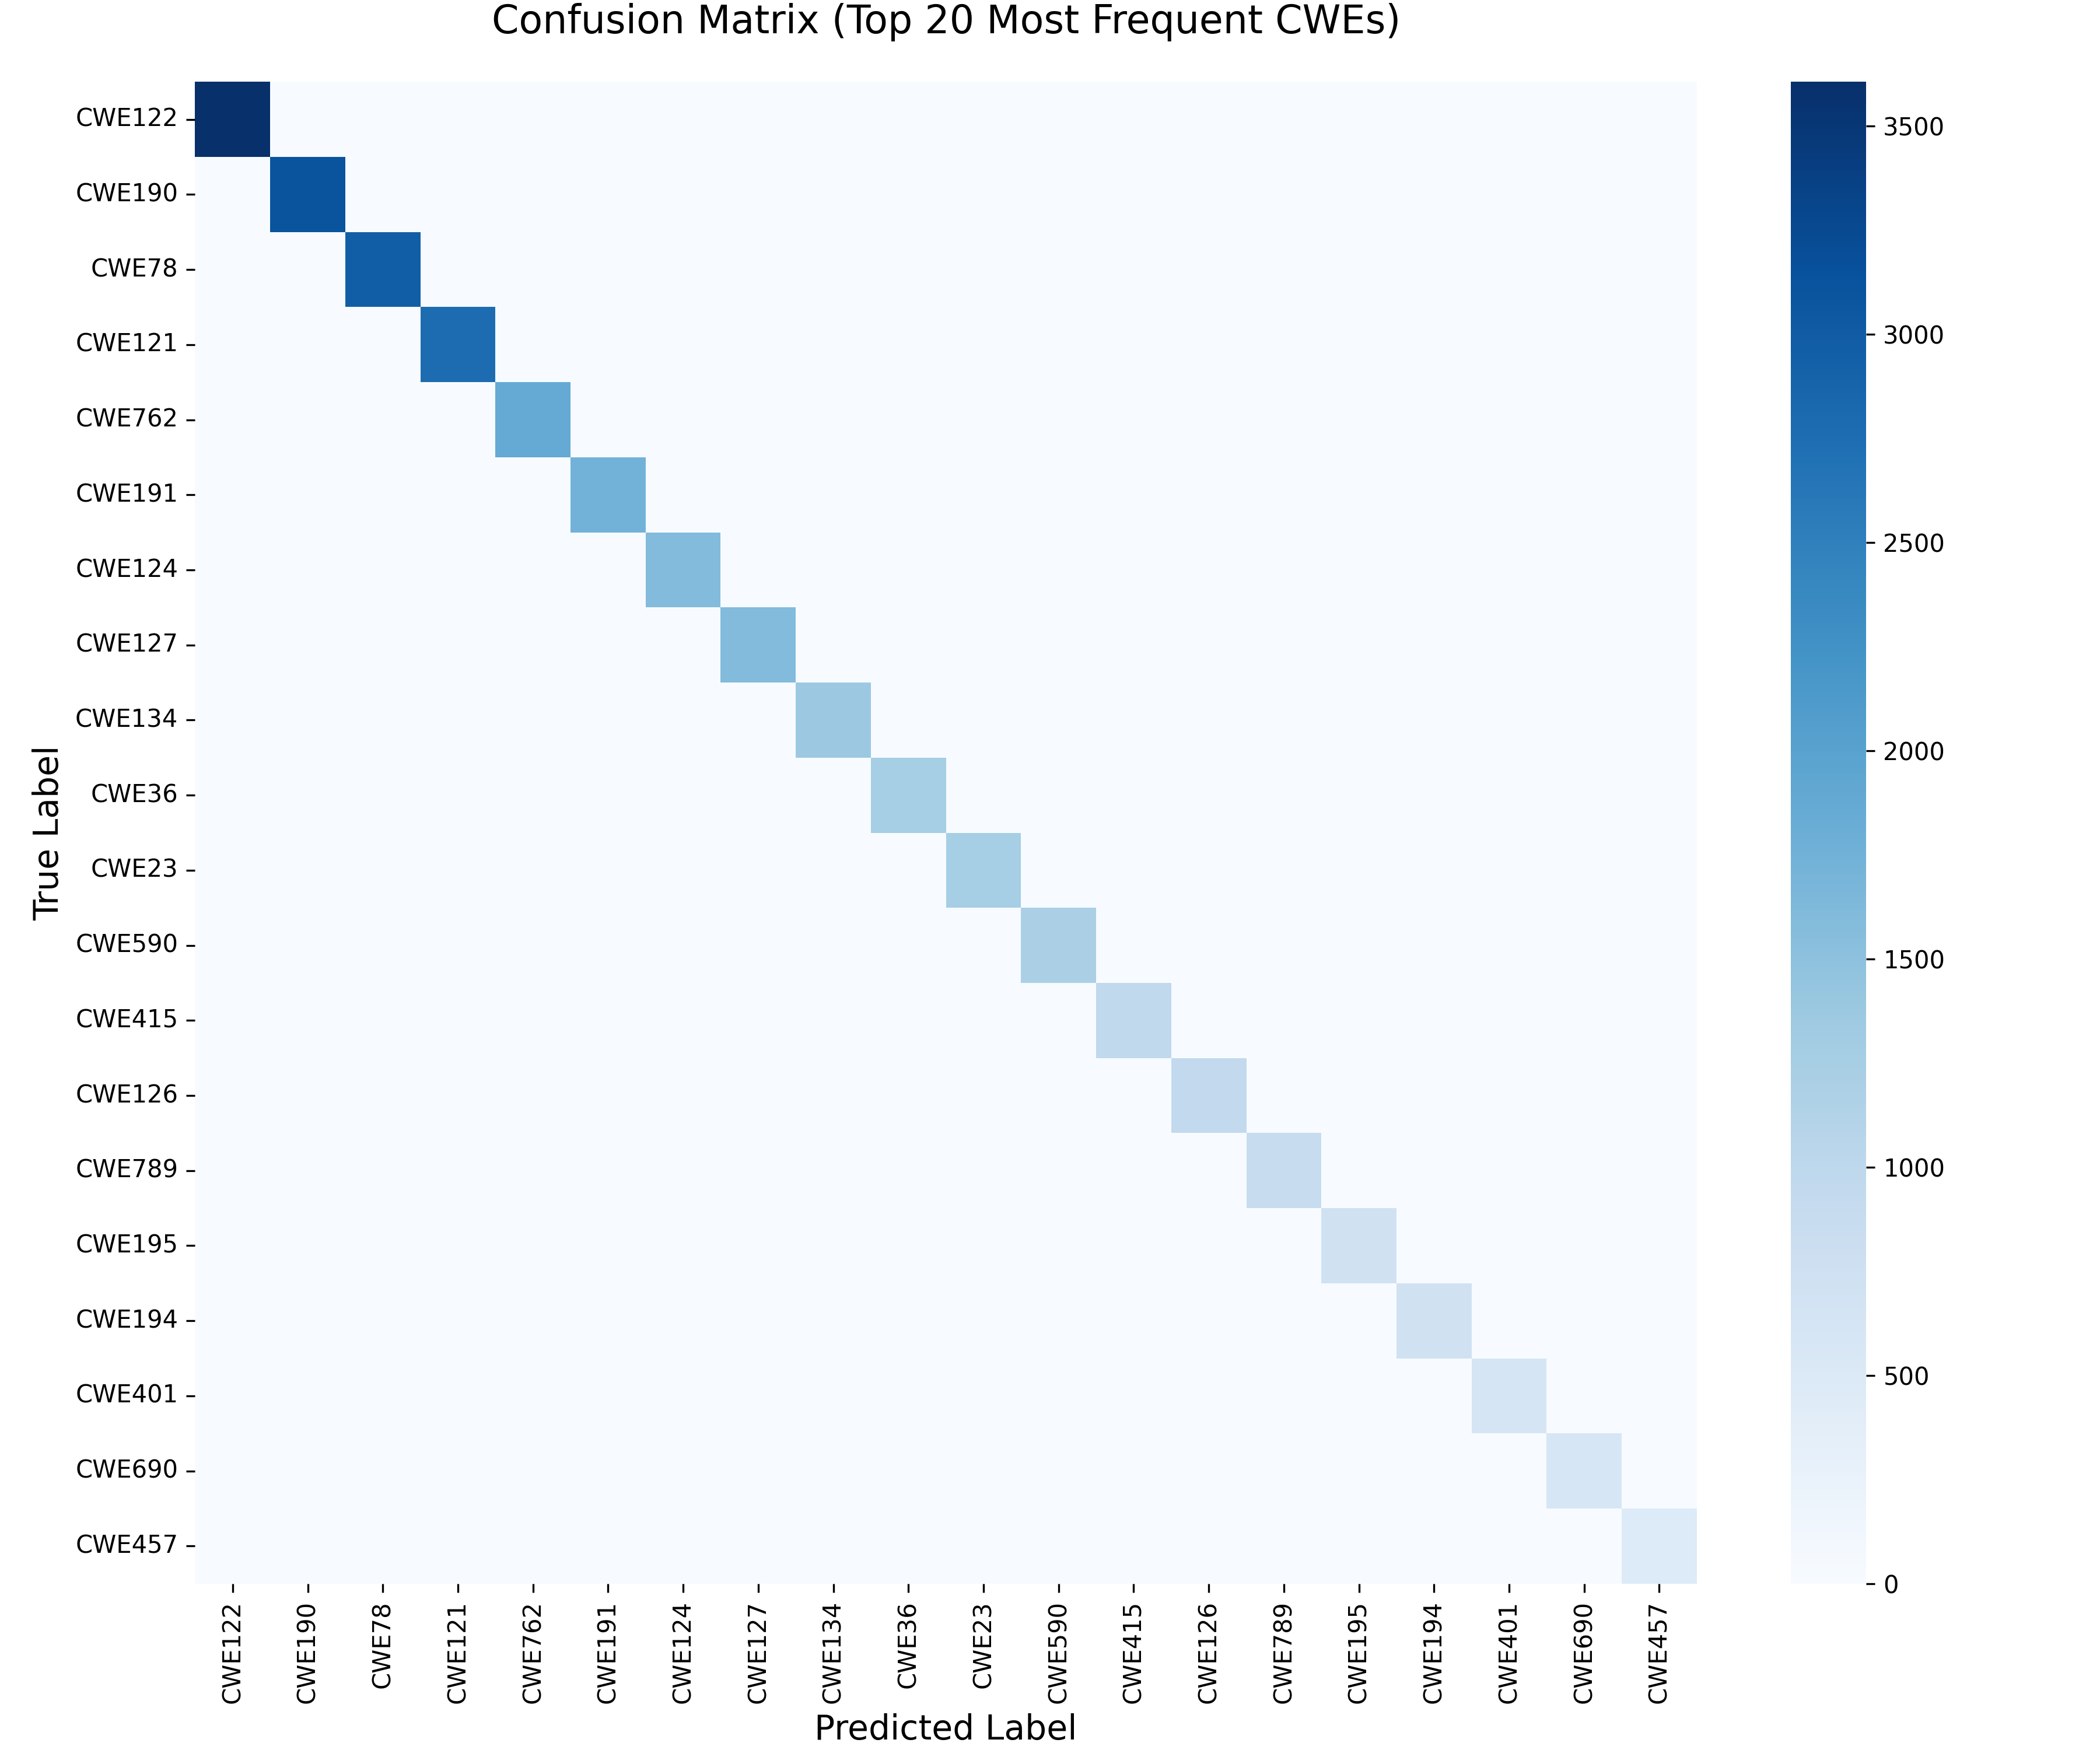
\includegraphics[width=0.48\textwidth]{confusion.png}
\caption{Confusion matrix for the ten most frequently occurring CWE categories in the Juliet dataset. These categories were selected due to their sufficient sample representation, allowing clearer visualization of inter-class confusion patterns and common misclassification trends.}
\label{fig:confusion}
\end{figure}
\subsection{Error Analysis}

To better understand the limitations of the proposed model, an analysis of the most frequently confused CWE categories is conducted.



Several CWE categories are frequently confused with one another due to similarities in their coding patterns and structural characteristics. Vulnerabilities that share overlapping features—such as memory handling errors and boundary-related issues—often exhibit similar code structures, making them difficult for the model to distinguish accurately.

The results confirm that misclassification occurs primarily because of closely associated vulnerability types rather than random prediction mistakes. These errors are systematic and indicate limitations in capturing fine-grained semantic differences between related classes.

Future improvements may involve incorporating additional semantic features, such as control flow and data flow information, as well as leveraging structural program representations to better differentiate between closely related vulnerability categories.

\subsection{Detailed Error Analysis}

A detailed analysis of misclassified samples reveals that most errors occur between semantically similar CWE categories. These vulnerabilities often share overlapping coding patterns, making it difficult for the model to distinguish between them.

Additionally, classes with very few training samples exhibit higher misclassification rates due to insufficient learning signals. This highlights the impact of dataset imbalance on classification performance.

The analysis confirms that the majority of errors are systematic rather than random, suggesting that improvements in data representation and class balancing techniques can significantly enhance model performance.
% =====================================================
\section{Class Imbalance Analysis}

The dataset exhibits extreme class imbalance across all 118 CWE categories. Major challenges arising from this imbalance include:
\begin{itemize}
    \item Dominance of majority classes during model training
    \item Insufficient training samples for minority vulnerability classes
    \item Biased predictions favouring well-represented categories
\end{itemize}

This imbalance reflects the long-tailed vulnerability distribution present within the benchmark dataset. Supervised learning models face significant difficulties because long-tailed distributions restrict training signals from rare categories. These findings highlight the importance of balanced dataset design and the use of macro-averaged metrics for fair evaluation.

% =====================================================
\section{Computational Efficiency}

The proposed CodeT5-small model contains approximately 60 million parameters, compared to 125 million parameters for CodeBERT and 220 million parameters for CodeT5-base.

The reduced parameter count also lowers memory requirements and improves deployment practicality, making the proposed framework suitable for automated vulnerability detection workflows.
The proposed framework demonstrates that effective vulnerability detection can be achieved with significantly lower computational requirements than larger transformer models. CodeT5-small requires approximately half the memory footprint of CodeBERT and a quarter of CodeT5-base, while still achieving strong classification performance across 118 CWE categories.

Training required approximately 2–3 hours per epoch using a batch size of 4 on a GPU-accelerated setup. Inference requires only a few milliseconds per code sample, enabling practical deployment in automated vulnerability scanning pipelines. The results confirm that lightweight transformer systems can balance efficiency and classification capability, The results demonstrate that lightweight transformer models can provide a practical balance between computational efficiency and vulnerability classification performance.

% =====================================================
\section{Discussion}

The findings highlight the effectiveness of transformer-based models for software vulnerability detection. Key insights from this work are:
\begin{itemize}
    \item Lightweight transformer models can achieve high performance while avoiding the computational overhead of large-scale architectures.

    \item Dataset design---in particular the choice of splitting strategy---significantly impacts evaluation reliability and overall model behaviour.

    \item Most classification errors are primarily driven by class imbalance rather than genuine confusion between vulnerability patterns.
\end{itemize}
The results also demonstrate that transformer models are capable of learning generalized representations of code rather than memorizing specific patterns. This ability is crucial for real-world deployment, where unseen and evolving vulnerabilities are common.

The transformer's ability to transfer pretrained semantic knowledge to new vulnerability patterns underscores the value of pretraining on large code corpora. This approach enables the model to identify vulnerability characteristics rather than merely memorizing specific code instances.
 Real-world codebases often contain noisy, incomplete, and highly diverse patterns, which may challenge the robustness of the model.
\subsection{Limitations}

Despite strong performance, the model is evaluated on a synthetic dataset that may not fully capture the complexity of real-world software systems.
% =====================================================
\section{Limitations and Future Work}
While the proposed transformer-based CWE classification system achieves strong performance, several directions can further enhance its effectiveness and practical applicability.

Although the present study focuses on the Juliet Test Suite, future work will extend the evaluation to real-world datasets such as Devign and Big-Vul to further validate generalization capability under diverse software development conditions.

\begin{itemize}

\item \textbf{Evaluation on Real-World Datasets:}  
The current work relies on the Juliet Test Suite, which contains synthetic vulnerabilities. Future work will involve evaluating the model on real-world datasets such as Devign, Big-Vul, and CVE repositories to assess robustness under noisy and diverse coding environments.

\item \textbf{Handling Severe Class Imbalance:}  
Although weighted loss functions improve performance, minority classes remain challenging. Advanced techniques such as focal loss, data augmentation, and few-shot learning can be explored to improve classification of rare vulnerabilities.

\item \textbf{Incorporating Program Structure:}  
The current model uses sequence-based representations of code. Future improvements can integrate structural information such as Abstract Syntax Trees (AST), Control Flow Graphs (CFG), and Data Flow Graphs (DFG) to enhance semantic understanding.

\item \textbf{Hybrid Transformer Models:}  
Combining lightweight transformer models with graph-based neural networks may improve the detection of complex vulnerabilities that require deeper contextual reasoning.

\item \textbf{Explainability and Interpretability:}  
Developing explainable AI techniques will help understand model predictions and improve trust among developers by highlighting the code regions responsible for detected vulnerabilities.

\end{itemize}
% =====================================================
\section{Conclusion}

This paper presented a transformer-based approach for software vulnerability classification using the CodeT5-small model trained on the Juliet Test Suite. The results demonstrate that even a lightweight model can achieve high accuracy when trained on a large and well-structured dataset. The introduction of template-aware splitting helps avoid data leakage and provides a more reliable evaluation than conventional random splitting of model performance.

The analysis confirms that most classification errors arise from class imbalance rather than genuine similarity between code patterns, highlighting the critical importance of dataset design in machine learning systems for vulnerability detection. The proposed approach is computationally efficient and practically viable for integration into secure software development pipelines.

Overall, this study demonstrates the effectiveness of compact transformer models in understanding source code and identifying vulnerabilities. Future improvements can focus on handling minority classes more effectively and extending the approach to real-world datasets for broader validation.

% =====================================================
\begin{thebibliography}{00}

\bibitem{codebert}
Z. Feng et al.,
``CodeBERT: A Pre-Trained Model for Programming and Natural Languages,''
\emph{Findings of EMNLP}, pp. 1536--1547, 2020.

\bibitem{graphcodebert}
D. Guo et al.,
``GraphCodeBERT: Pre-Training Code Representations with Data Flow,''
\emph{Advances in Neural Information Processing Systems (NeurIPS)}, 2020.

\bibitem{codet5}
Y. Wang, W. Wang, S. Joty, and S. C. Hoi,
``CodeT5: Identifier-Aware Unified Pre-Trained Encoder-Decoder Models for Code Understanding and Generation,''
\emph{Proceedings of EMNLP}, pp. 8696--8711, 2021.

\bibitem{codet5plus}
Y. Wang et al.,
``CodeT5+: Open Code Large Language Models for Code Intelligence,''
\emph{arXiv preprint arXiv:2305.07922}, 2023.

\bibitem{vuldee}
V. Li, Y. Zou, S. Jin, Z. Chen, and H. Wang,
``VulDeePecker: A Deep Learning-Based System for Vulnerability Detection,''
\emph{Proceedings of the Network and Distributed System Security Symposium (NDSS)}, 2018.

\bibitem{code2vec}
M. Alon, S. Brody, O. Levy, and E. Yahav,
``Code2Vec: Learning Distributed Representations of Code,''
\emph{Proceedings of POPL}, 2019.

\bibitem{cc2vec}
R. Zhang, H. Zhu, J. Yang, and J. Sun,
``CC2Vec: Code Character Sequence Representation Learning,''
\emph{ICSME}, 2019.

\bibitem{chen2022}
N. Chen et al.,
``A Comprehensive Study of CodeBERT for Code Search and Code-Related Tasks,''
\emph{IEEE Transactions on Software Engineering}, 2022.

\bibitem{devign}
Y. Zhou, S. Liu, J. Siow, X. Du, and Y. Liu,
``Devign: Effective Vulnerability Identification by Learning Comprehensive Program Semantics via Graph Neural Networks,''
\emph{Advances in Neural Information Processing Systems (NeurIPS)}, 2019.

\bibitem{bigvul}
Z. Fan, X. Liu, Y. Zhang, and X. Chen,
``A C/C++ Code Vulnerability Dataset with Detailed Annotations,''
\emph{Proceedings of the Mining Software Repositories (MSR)}, 2020.

% -------- AMRITA REFERENCES --------

\bibitem{amrita1}
R. Vinayakumar, K. P. Soman, P. Poornachandran, and V. K. Menon,
``A Deep-dive on Machine Learning for Cyber Security Use Cases: Principles, Algorithms, and Practices,''
in \emph{Machine Learning for Computer and Cyber Security}, Springer, 2019.

\bibitem{amrita2}
R. Vinayakumar et al.,
``Deep Learning Approach for Intelligent Intrusion Detection System,''
\emph{IEEE Access}, vol. 7, pp. 41525--41550, 2019.

\bibitem{amrita3}
M. H. Babu, R. Vinayakumar, and K. P. Soman,
``A Short Review on Applications of Deep Learning for Cyber Security,''
\emph{arXiv preprint arXiv:1812.05499}, 2018.

\bibitem{amrita4}
R. Vinayakumar et al.,
``Robust Intelligent Malware Detection Using Deep Learning,''
\emph{IEEE Access}, vol. 7, pp. 46717--46738, 2019.

\bibitem{amrita5}
R. Vinayakumar et al.,
``Application of Deep Learning Architectures for Cyber Security,''
in \emph{Machine Learning for Computer and Cyber Security}, Springer, 2019.
\bibitem{amrita6}
P. Seshagiri, A. Vazhayil, and P. Sriram,
``AMA: Static Code Analysis of Web Page for the Detection of Malicious Scripts,''
\emph{Procedia Computer Science}, 2016.
% -------- OTHER REFERENCES --------

\bibitem{pathbased}
M. Alon, S. Zilberstein, O. Levy, and E. Yahav,
``A General Path-Based Representation for Predicting Program Properties,''
\emph{Proceedings of POPL}, 2019.

\bibitem{contextcode}
Q. Shi, K. Huang, and Y. Hu,
``Learning Contextualized Code Representations,''
\emph{ASE}, 2019.

\bibitem{msr2020}
Y. Karampatsis and C. Sutton,
``Maybe Deep Neural Networks Are the Best Choice for Modeling Source Code,''
\emph{MSR}, 2020.

\end{thebibliography}

\end{document}